

\tikzset{every picture/.style={line width=0.75pt}} %set default line width to 0.75pt        

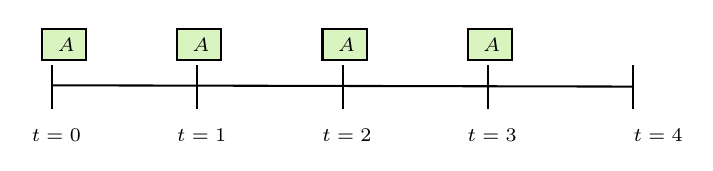
\begin{tikzpicture}[x=0.75pt,y=0.75pt,yscale=-1,xscale=1]
%uncomment if require: \path (0,300); %set diagram left start at 0, and has height of 300

%Straight Lines [id:da001] - Main timeline
\draw    (208.2,173) -- (487.68,173.61) ;
%Straight Lines [id:da002] - Vertical ticks
\draw    (208.2,163.27) -- (208.2,184.27) ;
\draw    (278.2,163.27) -- (278.2,184.27) ;
\draw    (348.2,163.27) -- (348.2,184.27) ;
\draw    (418.2,163.27) -- (418.2,184.27) ;
\draw    (488.2,163.27) -- (488.2,184.27) ;

%Shape: Rectangle [id:dp001] - Payment at t=0
\draw  [fill={rgb, 255:red, 184; green, 233; blue, 134 }  ,fill opacity=0.52 ] (203.53,145.73) -- (224.81,145.73) -- (224.81,160.73) -- (203.53,160.73) -- cycle ;
%Shape: Rectangle [id:dp002] - Payment at t=1
\draw  [fill={rgb, 255:red, 184; green, 233; blue, 134 }  ,fill opacity=0.52 ] (268.53,145.73) -- (289.81,145.73) -- (289.81,160.73) -- (268.53,160.73) -- cycle ;
%Shape: Rectangle [id:dp003] - Payment at t=2
\draw  [fill={rgb, 255:red, 184; green, 233; blue, 134 }  ,fill opacity=0.52 ] (338.53,145.73) -- (359.81,145.73) -- (359.81,160.73) -- (338.53,160.73) -- cycle ;
%Shape: Rectangle [id:dp004] - Payment at t=3
\draw  [fill={rgb, 255:red, 184; green, 233; blue, 134 }  ,fill opacity=0.52 ] (408.53,145.73) -- (429.81,145.73) -- (429.81,160.73) -- (408.53,160.73) -- cycle ;
% Text Node - Time labels
\draw (197,192.4) node [anchor=north west][inner sep=0.75pt]  [font=\scriptsize]  {$t=0$};
\draw (267,192.4) node [anchor=north west][inner sep=0.75pt]  [font=\scriptsize]  {$t=1$};
\draw (337,192.4) node [anchor=north west][inner sep=0.75pt]  [font=\scriptsize]  {$t=2$};
\draw (407,192.4) node [anchor=north west][inner sep=0.75pt]  [font=\scriptsize]  {$t=3$};
\draw (487,192.4) node [anchor=north west][inner sep=0.75pt]  [font=\scriptsize]  {$t=4$};

% Text Node - Payment labels
\draw (209.53,148.93) node [anchor=north west][inner sep=0.75pt]  [font=\scriptsize]  {$A$};
\draw (274.53,148.93) node [anchor=north west][inner sep=0.75pt]  [font=\scriptsize]  {$A$};
\draw (344.53,148.93) node [anchor=north west][inner sep=0.75pt]  [font=\scriptsize]  {$A$};
\draw (414.53,148.93) node [anchor=north west][inner sep=0.75pt]  [font=\scriptsize]  {$A$};


\end{tikzpicture}
